\chapter{Background}
\section{Machine Learning}
Machine learning is a sub-field of AI, which studies the development of systems that learn from experience without being explicitly programmed. There are different machine learning approaches, including supervised, unsupervised, and reinforcement learning, which describe what information is provided to the system and the method by which it learns from that information. This section gives an overview of supervised and reinforcement learning, as well as the basics of neural networks and their interpretability limitations.

\subsection{Supervised Learning}
Supervised learning is the most popular and successful machine learning approach, in which an algorithm learns to solve a problem by being exposed to example solutions to that problem. Specifically, the algorithm is given a collection of inputs and corresponding outputs (labels). This collection is called training data and each input-output pair is called a training example. The algorithm, then, automatically infers a mapping between those inputs and outputs through a process called training, after which it is able to assign labels to inputs it has not seen before. Different algorithms use different training methods, and this section will focus on Neural Networks, one of the most popular class of such algorithms.

\subsection{Neural Networks}
A Neural Network (NN), is a ML algorithm used widely for supervised learning. This section provides an overview of the standard, feed-forward NN architecture, but note that there are various types of NNs with different architectures and methods of training.

\subsubsection{High-Level Representation}
Neural networks are commonly represented as a set of successive layers: one input layer, one or more hidden layers, and one output layer. Each of those layers consists of a set of nodes and each of those nodes is connected to every node of the successive layer. A graphical representation of this structure can be seen in figure \ref{fig:neural_network}. The nodes in the input layer of such a network represent the set of properties (features) that describe the object that the NN is meant to classify. For example, in the classic problem of recognising handwritten digits (see, for example, \cite{handwritten}) images of handwritten digits are 'shown' to the network, by assigning a numerical value to each pixel in an image and using those as features. Each node in the input layer, then, corresponds to one of those features. Every node in the input layer passes its value, along with a numerical weight that represents the significance of that value, to every node of the first hidden layer. Each node in a hidden layer represents a mathematical function, which performs an arithmetic operation on the inputs and weights it receives from the previous layer and produces an output, which it passes on to every node of the next layer, along with a new corresponding weight. This process repeats until the initial input values have propagated through and been manipulated by each of the hidden layers in succession. The values produced by the final hidden layer pass on to the output layer, which performs the final calculation before providing an output which represents the network prediction about the input it was shown. In the case of the handwritten digit recognition problem, there are 10 nodes in the output layer (one for each digit from 0-9), and the value of each node represents the network's confidence in the handwritten digit it was shown being the one represented by the corresponding node. The digit represented by the node with the highest value is chosen as the network's decision.

The goal of the training phase of a NN is to compute a set of weights such that the network makes as few wrong predictions as possible. The weights are initially set to arbitrary numerical values (usually random) and are slowly tuned to minimise the number of errors the NN makes. The result of this process is a set of optimal weights, which the NN can then use in the process described above to assign labels to inputs it has not seen before.

\begin{figure}[ht]
    \centering
    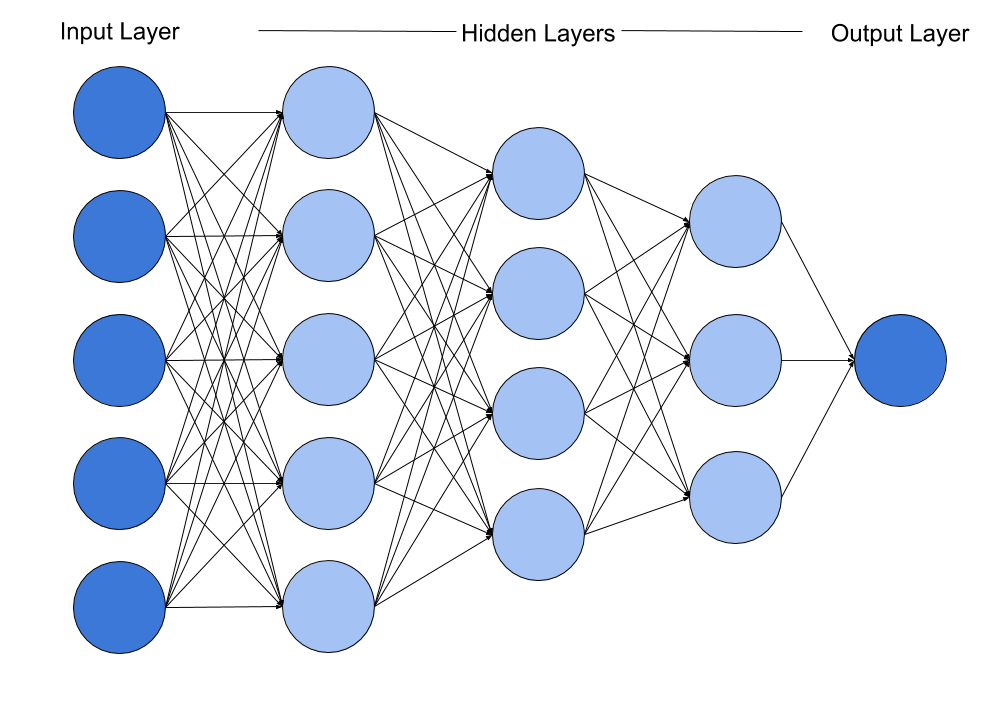
\includegraphics[width=12cm]{images/neural_network.png}
    \caption{Graphical representation of a feed-forward neural network with 3 hidden layers}
    \label{fig:neural_network}
\end{figure}

\subsection{Reinforcement Learning}
Reinforcement learning describes a process in which an algorithm (such as a neural network) plays the role of an agent that attempts to learn to operate in an environment by repeatedly interacting with it. The term "reinforcement" comes from the fact that the agent is provided with feedback from the environment, which comes in the form of a positive or negative reward depending on whether the agent is behaving in a way that brings it closer to achieving whatever goal the environment in question has set. The most intuitive example of such a setup is a video game, where the reward is the score the agent achieves by playing the game.

Similarly to supervised learning, the algorithm is provided with some input (the environment state) and learns to map it to some output (an action) such that some success metric (the reward) is optimised. However, in reinforcement learning, the algorithm is not provided with examples of correct input-output pairs. Instead, it has to actively interact with the environment to discover new inputs and learn to respond to them.

The process of reinforcement learning takes the form of an iterative experiment with some termination criteria. At the beginning of the experiment, the agent receives an encoded version of the initial state of the environment as input and outputs a random action, as it has no notion of which actions are going to yield maximum reward yet, which updates the state of the environment. Then, the environment provides the agent with a numerical reward (a positive or negative number representing reinforcement and punishment respectively) and the updated state. This process repeats until the agent achieves some predefined goal (e.g. wins the game) or one of the termination criteria is met (e.g. a timer runs out).

Like in supervised learning, neural networks are the most widely used algorithmic technique in reinforcement learning. In fact, the use of neural networks has given rise to a sub-field of reinforcement learning referred to as Deep Reinforcement Learning, which is characterised by the use of neural networks with multiple hidden layers.

\subsection{Uninterpretability of Machine Learning Models}
Since this project aims to propose a solution to the uninterpretability problem of current ML models, it is necessary to articulate clearly what uninterpretability means in this context and why these models suffer from it.

The simplest algorithm that is considered to belong to the set of ML models is linear regression. Linear regression is a statistical technique that attempts to infer a linear correlation between one or more variables. The result of applying this technique to a collection of concrete values for the variables in question is a linear model that "fits" the given data such that the error generated by predictions on the data using this model is minimal. The problem with this technique and, in fact, any statistical technique, is that it tells us nothing about the cause of the inferred relationship between the variables. That is to say, we know how the variables are correlated, but we don't know why that is, or what the exact relationship between them is. Take the popular problem of predicting house prices \cite{housing} as an example. Given a set of house characteristics along with the price each house was sold for, a model can be trained to predict the prices of houses it has not seen before. However, the model can tell us nothing about why, say, increasing the number of bedrooms tends to be correlated with an increase in price; it can merely tell us that, based on the available data, this seems to be the case. 

Neural networks are essentially more complex versions of traditional statistical techniques. This added complexity only serves to compound the problem of uninterpretability by increasing the number of transformations the original data undergoes to produce predictions, as well as the number of parameters the model requires to tune to make those predictions more accurate. Put simply, the only information the model provides us with is a table of floating-point numbers and a series of algebraic calculations that produce the prediction. This makes it impossible for humans to understand the reasoning behind the "decisions" a neural network makes, since they always take the form of statistical predictions. 

We might often be tempted to attribute reasoning to neural networks that perform high-level tasks, such as a neural network learning to play a video game via reinforcement learning, but this is an illusion: all the network does is receive encoded inputs, perform some calculations on them, and output the result, which the neural network predicts will produce an action in the video game that will bring it closer to the predefined "win" condition.

\section{Genetic Programming}
Genetic programming (GP) is a technique that borrows concepts from biological evolution to automatically generate programs that solve a specific problem. The algorithm generates an initial population of random programs and progressively modifies them until a program that can solve the problem in question emerges. GP takes the form of an iterative process in which the programs are repeatedly evaluated using a procedure (fitness function) to compute a measure of their performance. Then, a set of operations called genetic operations are performed on the population to produce a new generation of programs that are likely to perform better than their predecessors.

The characteristics of GP algorithms can be mapped to the components of a reinforcement learning agent to allow GP to be used on reinforcement learning tasks. Specifically, programs in a population can take the form of functions that take an environment state as input and produce an action as output. Subsequently, the reward provided by the environment can be used as the fitness measure for the programs, using which the algorithm can pick programs that perform well and discard the ones who don't. This mapping makes it possible to apply GP to reinforcement learning tasks.

\subsection{Program Structure}
In order to generate programs, the GP algorithm uses a domain-specific language (DSL) which is a language designed with the characteristics of the given problem in mind, as opposed to a general-purpose language which is designed to describe programs for any problem. The DSL consists of a function set and a terminal set. The function set contains the names of all the functions that can be used to construct programs and the terminal set contains variables and constants (terminals) that can be given as inputs to these functions. 

In the case of a typed DSL, each function takes a fixed number of arguments, each of which has to be of a specific type (e.g. 'number' or 'string'). The amount of arguments a function takes is known as its arity. Therefore, when constructing programs using this language, the GP algorithm has to ensure that the number of terminals chosen as the arguments to a function matches its arity, and that the type of each terminal matches that of the corresponding argument. If a function produces an output, then that also has a type, which must be checked when a function is passed as an argument to another function. If the DSL is untyped, any function can take any terminal or other function as an argument without any restrictions.

\subsection{Tree-Based Program Representation}
Programs generated by a GP algorithm can be represented as trees. The root (top) node of the tree represents a function, and each of its branches represents an argument to that function. If a branch leads to a node with more branches (sub-tree), then this is also a function. Eventually, every sub-tree has to reach a node that has no branches, called a leaf, and each leaf represents a terminal (e.g. a number) that is passed as an argument to the function represented by the root of the sub-tree that leaf is connected to. For example, figure \ref{fig:example_program_tree} shows a visual representation of a program that consists of a function, \verb+IFLTE+ (if-less-than-or-equal), which takes four arguments: three terminals (\verb+pa+, \verb+0+, and \verb+R+) and another \verb+IFLTE+ function which takes four terminals (\verb+pv+, \verb+0+, \verb+L+, and \verb+R+) as its arguments.

\begin{figure}[ht]
    \centering
    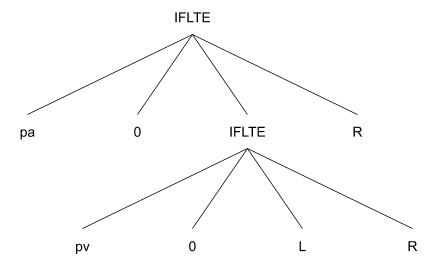
\includegraphics[width=10cm]{images/complex_iflte_program.png}
    \caption{Tree representation of an example program produced by a GP algorithm.}
    \label{fig:example_program_tree}
\end{figure}

\subsection{Genetic Operators}
Genetic operators are algorithms that take one or more programs from a population as input and generate a new program as output. The three main types of genetic operators are selection, mutation and crossover. Selection is the simplest of the three and is commonly used to pick programs from the population to be used by the other two operators. There are many different selection algorithms, two of the most popular being fitness proportionate selection (aka roulette wheel selection) and tournament selection. Fitness proportionate selection uses a pseudorandom number generator to select programs from a population such that the higher the fitness of a program, the higher the probability that program will be chosen. Tournament selection randomly selects a subset of the programs in a population (the size of the subset is called tournament size) and picks the program with the highest fitness; the higher a program's fitness, the higher its probability of "winning" any of the tournaments it's placed in. Tournament selection provides more flexibility than fitness proportionate selection because it's possible to adjust the probability of weak individuals being selected (selection pressure) by increasing or decreasing the tournament size. Decreasing the selection pressure can be useful to avoid early convergence, i.e. the fittest programs of the first few generations dominating the population and not allowing better programs to emerge.

The mutation operator randomly selects a proportion of the programs in the population, and changes one of the program's sub-trees (in the case of tree-based representation) with a randomly generated sub-tree. The exact value of the proportion of the population that is selected for mutation is called the mutation rate of the algorithm.

Finally, crossover attempts to simulate a simple version of biological sexual reproduction. It selects two programs (parents) from the population using the selection operator, randomly picks a node on each of them (crossover point) and then combines the sub-trees that have the chosen node as their root to create a new program (offspring). The proportion of programs generated using crossover is called the crossover rate. Crossover was not used in this project for the sake of simplicity, as it did not prove necessary for the generation of programs that served as good solutions to the problems tackled.

\section{Related Work}
The problem of the uninterpretability of ML models has been known for a long time and a lot of research has been done to address the issue. Additionally, Genetic Programming has been a useful optimisation technique since its establishment with papers such as \cite{koza}, from which this project borrowed the idea for the \verb+IFLTE+ function, which served as the primary building block for the solutions produced and discussed in this report. Recently, there have been quite a few attempts to integrate Genetic Algorithms (of which GP algorithms are a subset) into the ML workflow, as seen for example in \cite{relatedwork1}, \cite{relatedwork2} and \cite{relatedwork3}, as well as attempts to use GP (e.g. \cite{gprl}, \cite{pirl}, \cite{atari}) to make solutions to ML problems more interpretable. To my knowledge, however, all of these approaches either use neural networks in some fashion, thus inevitably trading interpretability for performance, or use GP as a black-box algorithm whose solutions are no more interpretable than those produced by a neural network.

In this project, GP was used directly to attempt to solve problems that are traditionally solved using black-box ML models. The solutions produced take the form of human-readable programs that use familiar logical structures and high-level representations of the problem parameters to make them interpretable. The hope is that this will allow us to reason about solutions to these problems, instead of merely relying on the robustness of the black-box models that produce them.
